\chapter{Introducción}
\label{ch1}

%%%%% https://cerncourier.com/a/pushing-the-precision-frontier/
% https://home.cern/news/news/physics/why-precision-luminosity-measurements-matter
La física de partículas es una rama de la física que se dedica al estudio de las partículas fundamentales y las fuerzas que constituyen la materia y la radiación en el universo. El Modelo Estándar clasifica a las partículas fundamentales y sus interacciones en dos grandes categorías: los fermiones, que son las partículas que forman la materia, y los bosones, que son las partículas responsables de transmitir las fuerzas fundamentales. Para investigar estas interacciones, se utilizan aceleradores de partículas de alta energía, los cuales permiten medir diversos parámetros y propiedades de las partículas generadas en las colisiones. En este capítulo, se presenta una visión general de las partículas elementales, los colisionadores de partículas y la evaluación de su rendimiento, destacando los conceptos y definiciones clave que son esenciales para la comprensión de este proyecto de tesis.

\section{Física de Partículas y el Modelo Estándar}

El universo está formado por una variedad de partículas diferentes. Los átomos, por ejemplo, están constituidos por electrones ($e$\textsuperscript{-}) con carga negativa, que se encuentran en estado ligado orbitando alrededor de un núcleo central. Este núcleo está compuesto por protones $(p)$, que poseen carga positiva, y neutrones $(n)$, que son eléctricamente neutros. Los electrones se mantienen unidos al núcleo debido a la atracción electrostática entre sus cargas opuestas, mientras que los protones y neutrones están cohesionados por la fuerza nuclear fuerte. Además de estas interacciones, también influyen la gravedad y la fuerza débil. La fuerza débil es responsable de fenómenos como la radiactividad nuclear, mientras que la gravedad, aunque extremadamente débil en comparación con las otras fuerzas, es la que determina la estructura del universo a gran escala debido a su naturaleza atractiva universal \cite{thomson_2013}. 

A pesar de que este modelo físico es útil para describir la materia a bajas energías, cuando se exploran escalas de energía más altas, se descubren estructuras mucho más complejas. Este tipo de estudios ha permitido identificar 17 partículas fundamentales que constituyen la totalidad del universo conocido. Estas partículas se dividen en dos categorías principales: los fermiones, que son las partículas que forman la materia y tienen un espín de $1/2$, y los bosones, que son los mediadores de las fuerzas fundamentales y presentan un espín entero.

Comenzando con los fermiones, estos componenen a la materia en el universo y estos consisten en doce partículas fundamentales las cuales se clasifican en dos grupos: leptones y quarks. A su vez, estos se organizan en tres generaciones,

La materia está compuesta por fermiones, que incluyen un total de doce partículas fundamentales, divididas en dos tipos: los leptones y los quarks. Estas partículas se agrupan en tres generaciones, donde los miembros de generaciones superiores poseen una mayor masa que sus contrapartes en las generaciones anteriores. Los seis leptones se dividen en tres partículas con carga: el electrón ($e$\textsuperscript{-}), el muón ((${\mu}$\textsuperscript{-}), y el tau (${\tau}$\textsuperscript{-}), junto con sus correspondientes neutrinos: el neutrino electrónico ($\nu_{e}$), el neutrino muónico ($\nu_{\mu}$), y el neutrino tau ($\nu_{\tau}$). 

Por otro lado, los quarks solo existen confinados dentro de hadrones, y su grupo está compuesto por seis tipos: el quark arriba ($u$), quark abajo ($d$), quark encanto ($c$), quark extraño ($s$), quark cima ($t$) y quark fondo ($b$). Las propiedades de estas doce partículas fundamentales se detallan en la Tabla 1.1, proporcionando una visión general de sus características y su papel en la estructura de la materia.

\begin{table}[h!]
	\begin{center}
%\centering
	\caption[Los doce fermiones fundamentales y sus propiedades]{Los doce fermiones fundamentales y sus propiedades}
		\label{tab:table1}
		\begin{tabular}{lllrcllrc}
                                                                                & \multicolumn{4}{c}{\textbf{Leptones}}                                                                     & \multicolumn{4}{c}{\textbf{Quarks}}                                                \\ 
%\cline{2-9}
 \midrule[1.1pt]
                            \multicolumn{1}{c}{Generación }& \multicolumn{2}{c}{Particula } & \multicolumn{1}{c}{\textit{Q}} & masa/GeV                          & \multicolumn{2}{c}{Particula} & \multicolumn{1}{c}{\textit{Q}} & masa/GeV  \\ 
\hline
\multirow{2}{*}{\begin{tabular}[c]{@{}l@{}}Primera\end{tabular}}  & electrón & ($e$\textsuperscript{-})                 & -1                             & 0.0005                            & down    & ($d$)                & -1/3                           & 0.003     \\
                                                                                & $e$-neutrino & ($\nu_{e}$)                 & 0                              & \textless{}10\textsuperscript{-9} & up      & ($u$)                & +2/3                           & 0.005     \\
\multirow{2}{*}{\begin{tabular}[c]{@{}l@{}}Segunda\end{tabular}} & muon     & (${\mu}$\textsuperscript{-})                 & -1                             & 0.106                             & strange & ($s$)                & -1/3                           & 0.1       \\
                                                                                & $\mu$-neutrino & ($\nu_{\mu}$)                 & 0                              & \textless{}10\textsuperscript{-9} & charm   & ($c$)                & +2/3                           & 1.3       \\
\multirow{2}{*}{\begin{tabular}[c]{@{}l@{}}Tercera\end{tabular}} & tau      & ({$\tau}$\textsuperscript{-})                 & -1                             & 1.78                              & bottom  & ($b$)                & -1/3                           & 4.5       \\
                                                                                & $\tau$-neutrino & ($\nu_{\tau}$)                 & 0                              & \textless{}10\textsuperscript{-9} & top     &($t$)                & +2/3                           & 174      
\end{tabular}
	\end{center}
		\end{table}

Los bosones son las partículas encargadas de mediar las interacciones entre los fermiones, a través del intercambio de partículas denominadas bosones gauge. La fuerza electromagnética es transmitida por el fotón ($\gamma$), mientras que la fuerza débil es mediada por los bosones $W^{\pm}$ y $Z^{0}$, y la fuerza fuerte por los gluones ($g$). También existe un bosón escalar, el bosón de Higgs, cuya función principal es conferir masa a las partículas fundamentales. La Tabla 1.2  presenta un resumen detallado de las fuerzas fundamentales que afectan a los fermiones, mostrando cómo estas fuerzas son transportadas por sus respectivos bosones mediadores.


\begin{table}[h!]
  \begin{center}
    \caption[Fuerzas experimentadas por los fermiones]{Fuerzas experimentadas por los fermiones.}
    \label{tab:table2}
    \begin{tabular}{l c c c c}
    &    &  \textbf{Electromagnetica} & \textbf{Débil} & \textbf{Fuerte}\\
      \midrule[1.1pt]
      \multirow{2}{*}{Leptones} & ${e}$\textsuperscript{-} \hspace{0.3cm}  ${\mu}$\textsuperscript{-} \hspace{0.3cm} ${\tau}$\textsuperscript{-} & \checkmark & \checkmark & \\ % <-- Combining 2 rows with arbitrary with (*) and content 12
      & $ \nu_{e} $ \hspace{0.3cm}  $\nu_{\mu}$ \hspace{0.3cm} $\nu_{\tau}$  &  & \checkmark\\ % <-- Content of first column omitted.
      \hline
      \multirow{2}{*}{Quarks} & $u$ \hspace{0.5cm}  $c$\hspace{0.5cm} $t$ & \checkmark & \checkmark& \checkmark\\
      & $d$ \hspace{0.5cm}  $s$\hspace{0.5cm} $b$ & \checkmark & \checkmark & \checkmark\\

    \end{tabular}
  \end{center}
\end{table}

Las partículas mencionadas están descritas dentro del Modelo Estándar de la física de partículas, el cual es, hasta ahora, la teoría más sólida para explicar con éxito los resultados experimentales. Sin embargo, la mayoría de estos datos provienen de colisionadores de partículas, ya que dichas partículas se pueden producir y estudiar cuando se generan colisiones a energías muy elevadas.

\section{Colisionadores de Partículas y Sección Eficaz de Producción}

En los últimos años, la física de partículas ha logrado grandes avances, impulsados por el uso de aceleradores de partículas de alta energía. Estos dispositivos funcionan como microscópicos muy poderosos, permitiendo examinar las estructuras más pequeñas de la materia y sus partículas fundamentales, tales como electrones, protones, neutrones, neutrinos y quarks. Además, los aceleradores de partículas ofrecen la posibilidad de resolver misterios sobre los componentes desconocidos del universo, como la materia y la energía oscura.\\

Los colisionadores de partículas aceleran haces de partículas cargadas a velocidades cercanas a la de la luz mediante el uso de campos electromagnéticos. Cuando estos haces chocan a altas energías, se producen interacciones llamadas eventos, en los que se generan varias partículas nuevas (como el bosón de Higgs). La mayoría de estas partículas no se pueden observar directamente, ya que se desintegran rápidamente en otras partículas. Sin embargo, los experimentos con detectores de partículas permiten medir e identificar estas partículas mediante tecnologías y diseños especializados, que se basan en las propiedades de las partículas y sus interacciones con la materia \cite{thomson_2013}.\\

Un detector de partículas se suele construir en forma de un barril cilíndrico o poligonal, colocado en paralelo con los haces que colisionan. Dos tapas planas en los extremos sellan la estructura, permitiendo una cobertura casi completa del ángulo sólido alrededor del tubo de haces. Este tipo de detector consta de varias capas, cada una diseñada para registrar diferentes partículas creadas durante las colisiones \cite{thomson_2013}.\\

Los colisionadores de partículas se miden principalmente por dos factores: la energía disponible en el centro de masas y la luminosidad, que es la tasa de colisiones. La cantidad de energía disponible para la creación de nuevas partículas es crucial, ya que define el rango de partículas que pueden producirse y estudiarse. Durante los experimentos, las partículas se aceleran y se dirigen unas contra otras, generando nuevas partículas e interacciones que luego pueden ser analizadas \cite{undergraduate_accelerators_chapter}.\\

Los colisionadores de haces enfrentados permiten alcanzar energías extremadamente altas en el punto donde los haces se cruzan. Cuando las partículas en los haces tienen la misma energía y un momentum opuesto (es decir, cuando las masas son iguales), el experimento tiene lugar en el marco de referencia del centro de masas (CM), lo que permite que toda la energía del acelerador se emplee para crear partículas de gran masa. En física de partículas, la cantidad invariante de Lorentz ($s$) se utiliza para representar el cuadrado de la energía total entrante, y se define como:

\begin{equation}
s = \left ( \sum_{i = 1,2}^{}E_{i} \right )^{2}-\left ( \sum_{i = 1,2}^{}p_{i} \right )^{2}c^{2}
\end{equation}

Donde \( p \) y \( E \) representan el momento y la energía de cada partícula entrante, respectivamente. En el sistema de referencia del centro de masas (CM), donde los momentos de las partículas son iguales pero de direcciones opuestas, el segundo término en la ecuación de la cantidad invariante de Lorentz (\( s \)) se anula. Como resultado, la expresión se simplifica a \( s = 4E^2 \), donde \( E \) es la energía de cada partícula en el marco del centro de masas. Esta simplificación es crucial para calcular la energía disponible en las colisiones de partículas \cite{undergraduate_accelerators_chapter}.\\

El segundo parámetro importante para evaluar el desempeño de los colisionadores es la luminosidad, que indica la capacidad del acelerador para generar suficientes interacciones. La luminosidad se determina a través de un factor de proporcionalidad entre la probabilidad cuántica de que ocurra una interacción (llamada sección eficaz) y la cantidad de eventos por segundo para un proceso físico específico ($R$) \cite{ref_lib_vol3}.\\

En física de partículas, el término sección eficaz tiene un significado especializado que difiere de su uso cotidiano. Mientras que normalmente "sección" hace referencia a una parte o corte de un objeto, en este contexto se refiere a la probabilidad de que dos partículas interactúen durante una colisión, expresada en metros cuadrados. Cuando dos haces de partículas chocan en un acelerador, pueden darse varios procesos, y la sección eficaz de cada uno depende del tipo y la energía de las partículas que colisionan.\\

Por ejemplo, en el Gran Colisionador de Hadrones (LHC), algunas partículas como los bosones  $W^{\pm}$ y $Z^{0}$ tienen secciones eficaces grandes, lo que hace más frecuentes sus observaciones. En cambio, el bosón de Higgs tiene una sección eficaz mucho menor, lo que complica su producción y detección.\\

Para comprender mejor este concepto, imaginemos un caso simple: un haz de partículas del tipo $a$ atraviesa una región donde hay partículas del tipo $b$. La tasa de interacciones entre estos dos tipos de partículas depende de la densidad de partículas $b$ por unidad de volumen, denotada como $n_{b}$, y del flujo de partículas incidentes $a$, representado por $\phi_{a}$ . La tasa de interacción por partícula objetivo $b$ se puede expresar de la siguiente forma:

\begin{equation*}
  r_{b}=\sigma \phi_{a}
\end{equation*}


El concepto central en la física fundamental se puede describir mediante la sección eficaz de interacción, simbolizada por $\sigma$. Este parámetro, que se mide en unidades de área, refleja la probabilidad de que una interacción tenga lugar entre una partícula incidente y una partícula objetivo. Para visualizarlo, se puede pensar que cada partícula objetivo tiene un área efectiva, y la sección eficaz de interacción corresponde a esa área. En la figura 1.1(a), se muestra una representación de este concepto, donde una partícula del tipo $a$, que viaja con velocidad $v_{a}$, se mueve a través de una región con área $A$, que contiene partículas del tipo $b$ con velocidad $v_{b}$ en dirección opuesta. El valor de la sección eficaz de interacción depende de la probabilidad cuántica de que ocurra la interacción, lo cual es esencial para entender cómo se comportan las partículas durante las colisiones \cite{thomson_2013}.

\begin{center}
  \begin{figure}[h!]
    \centering
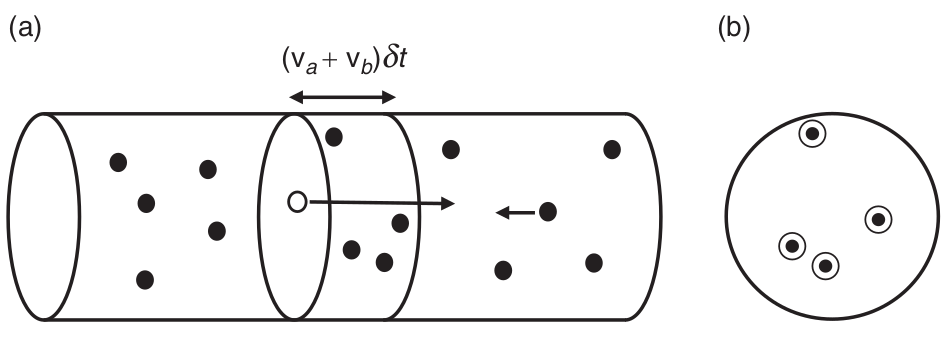
\includegraphics[scale=.35]{Chapter1/cross_section.png} 
 \caption[Ilustración de la sección eficaz]{Izquierda (a): haz incidente de partículas de tipo $a$ atravesando una región que contiente partículas de tipo $b$. Derecha (b):  vista proyectada de la región atravesada por la partícula incidente en un intervalo de tiempo $\delta t$.}
    \label{cross_section}
  \end{figure}
\end{center}

Para comprender la probabilidad de una interacción entre partículas de los tipos $a$ y $b$, supongamos que, durante un intervalo de tiempo $\delta t$, la partícula $a$ pasa a través de una región que contiene  $\delta N= n_{b}(v_{a}+v_{b}) A \delta t$ partículas de tipo $b$. La probabilidad de que ocurra una interacción se calcula dividiendo el área total efectiva de la sección transversal de las $\delta N$ partículas por el área $A$. Este cálculo puede interpretarse como la probabilidad de que la partícula incidente atraviese una de las regiones de área $\sigma$ que rodean a cada una de las partículas objetivo, tal como se muestra en la figura 1.1(b).

En este sentido, la sección eficaz de un proceso se define como el área efectiva asociada con el objetivo para ese proceso en particular, y se mide en unidades de área. Formalmente, se expresa mediante la ecuación 1.2.

\begin{equation}
\sigma=\frac{\text{número de interacciones por unidad de tiempo por partícula objetivo}}{\text{flujo incidente}}
\label{cross}
\end{equation}

%begin{equation}
%\sigma=\frac{\text{number of interaction per unit time per target particle}}{\text{incident flux}}
%\end{equation}

%\delta P= \frac{\delta N \sigma}{A}=\frac{n_{b}(v_{a}+v_{b})A\sigma \dela t}{A}= n_{b}v\sigma \delta t$
%where $v=v_{a}+v_{b}$. The interaction rate for each particle of type $a$ is $r_{a}= \frac{dP}{dt}= n_{b} v\sigma$.
%For a beam of particles of type $a$ with number density $n_{a}$ confined to a volume $V$, the total interaction rate is:
%$\text{rate}=r_{a}n_{a}V=(n_{b}v\sigma) n_{a}V= (n_{a}v)(n_{b}V)\sigma$

%$\text{rate}=(n_{a}v)(n_{b}V) \sigma = \phi N_{b} \sigma$

%Thus the total rate is equal to
%$\text{rate}= \text{flux} \times \text{number of target particles} \times \text{cross section}$

%More formally, the cross section for a process is defined as:
\section{Luminosidad }

En los experimentos de física de partículas, el número de interacciones útiles (o eventos) es tan crucial como la energía involucrada. La capacidad de un acelerador de partículas para generar estas interacciones se mide mediante un parámetro llamado "luminosidad instantánea" \( \mathcal{L}_{inst} \). Esta luminosidad es directamente proporcional al número de eventos producidos por segundo y a la sección eficaz \( \sigma_p \) del proceso de interés \cite{concept_of_luminosity}.

\begin{equation}
R=\mathcal{L}_{inst} \cdot \sigma_{p}
\end{equation}

Donde las unidades de la luminosidad son $cm^{-2}s^{-1}$. 

Para derivar una expresión general para la luminosidad en el caso de dos haces que colisionan, consideramos que ambos haces actúan simultáneamente como el objetivo y el haz incidente. Supondremos que los haces están "agrupados", es decir, que las partículas se organizan en paquetes o "bunches". 

En este escenario, cada paquete de partículas se considera como una región de alta densidad de partículas que interactúan entre sí. La luminosidad instantánea se puede entonces expresar en términos del número de partículas por paquete, el tamaño del paquete y la velocidad de los haces. El número de interacciones por unidad de tiempo dependerá tanto de la densidad de las partículas en los paquetes como de la sección eficaz de la interacción entre ellas.

\begin{center}
  \begin{figure}[h!]
    \centering
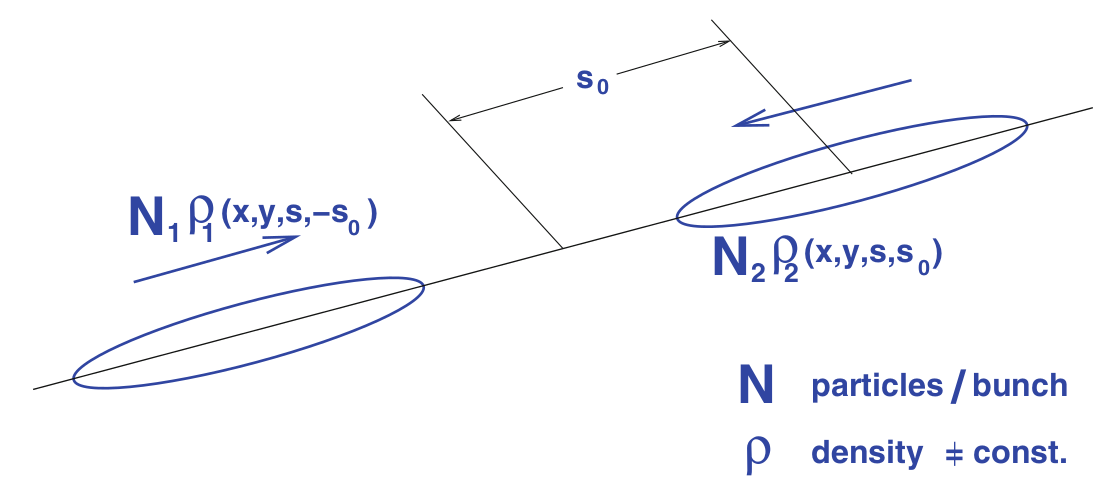
\includegraphics[scale=.25]{Chapter1/luminosity.png} 
 \caption[Interacción entre dos haces de partículas]{Esquema de una interacción entre dos haces de partículas\cite{concept_of_luminosity}.}
    \label{luminosity}
  \end{figure}
\end{center}

%A schematic picture is shown in Fig. \ref{luminosity}. Since the two beams are not stationary but are moving through each other, the overlap integral depends on the longitudinal position of the bunches, and therefore on time. As the beams move towards and through each other, the two beams have different distribution functions and a different number of particles in the beams \cite{concept_of_luminosity}. The overlap integral, which is proportional to the luminosity $\mathcal{L}_{inst}$, can then be written as:


En la Figura 1.2 se muestra un diagrama que ilustra cómo dos haces se intersectan entre sí. Dado que estos haces no están estáticos, sino en movimiento, la forma en que se superponen depende del tiempo y la posición de los paquetes de partículas. Mientras los haces se desplazan, también tienen distribuciones y números de partículas diferentes en su interior \cite{concept_of_luminosity}.

La luminosidad instantánea  \( \mathcal{L}_{inst} \) , que es proporcional a la integral de superposición de los haces, se puede expresar de la siguiente manera:
 
\begin{equation}
  \mathcal{L}_{inst}\propto K\cdot \int\int\int \int_{-\infty}^{\infty} \rho_{1}(x,y,s,-s_{0}) \rho_{2}(x,y,s,s_{0})dxdydsds_{0}
    \label{lumi_1}
\end{equation}
 
Donde las funciones $\rho_{1}(x,y,s,-s_{0})$ y $\rho_{2}(x,y,s,s_{0})$ representan la distribución de densidad del haz en un tiempo $t$. Ahora, asumimos que los bunches interaccionan en el punto $s_{0} = 0$. Debido a que los haces estan en movimiento y en dirección contraria, debemos considerar un factor cinético relativista de la forma:

\begin{equation}
 K = \sqrt{(\vec{v_{1}}-\vec{v_{2}})^{2}-(\vec{v_{1}}\times \vec{v_{2}})^{2}/c^{2}}
    \label{kinematic}
\end{equation}

Cuando los paquetes de partículas colisionan de manera frontal y se desplazan casi a la velocidad de la luz, el factor cinético relativista toma un valor de 2.

Asumiendo que las densidades son no correlacionadas en todos los planos y que las colisiones son frontales, donde las velocidades de los dos paquetes son opuestas $(\vec{v_{1}}=-\vec{v_{2}})$, la integral de superposición puede factorizarse de la siguiente manera:


\begin{equation}
  \mathcal{L}_{inst}= 2N_{b} N_{1}N_{2}f \int\int\int\int_{-\infty}^{\infty}  \rho_{1x}(x)\rho_{1y}(y)\rho_{1s}(s-s_{0})\rho_{2x}(x)\rho_{2y}(y)\rho_{2s}(s+s_{0}) dxdydsds_{0}
    \label{luminosity_2}
\end{equation}

donde $N_{b}$ es el número de bunches en un haz, $N_{1}$ y $N_{2}$ son las particulas por bunche y $f$ la frecuencia de revolución.\\



%\begin{eqnarray}
%\rho_{iz}(z)= \frac{1}{\sqrt{2\pi} \sigma_{z}} exp \biggl(-\frac{z^{2}}{2\sigma_{z}^{2}} \biggr)&z=x,y&i=1,2 
%\end{eqnarray}

%\begin{eqnarray}
%\rho_{s}(s\pm s_{0})= \frac{1}{\sqrt{2\pi} \sigma_{s}} exp \biggl(-\frac{(s\pm s_{0})^{2}}{2\sigma_{s}^{2}} \biggr)
%\end{eqnarray}

Suponiendo perfiles gaussianos en todas las dimensiones y longitudes de los paquetes aproximadamente iguales $(\sigma_{1s}\approx \sigma_{2s})$, la ecuación (1.6) se puede resolver para obtener la luminosidad instantánea en función de la superposición de los haces \cite{concept_of_luminosity}.

Para el caso general en el que $\sigma_{1x}\neq \sigma_{2x}$ y $\sigma_{1y}\neq \sigma_{2y}$, las distribuciones de densidad de las partículas en los planos $x$ y $y$ serán diferentes. En este caso, la integral de superposición debe tener en cuenta las diferentes dispersión de los haces en las direcciones transversales, lo que implica que las ecuaciones para calcular la luminosidad instantánea se vuelve mas compleja.


\begin{equation}
  \mathcal{L}_{inst}= \frac{N_{1} N_{2} N_{b}f }{2\pi \sqrt{\sigma_{1x}^{2}+\sigma_{2x}^{2}}\sqrt{\sigma_{2y}^{2}+\sigma_{2y}^{2}}}
  \label{lumi_general}
\end{equation}

Asumiendo haces iguales, $\sigma_{1x}= \sigma_{2x} \text{ y } \sigma_{1y}= \sigma_{2y}$:

\begin{equation}
  \mathcal{L}_{inst}= \frac{N_{1} N_{2} N_{b}f }{4\pi \sigma_{x} \sigma_{y}}
  \label{lumi_theor}
\end{equation}

Esta expresión es ampliamente reconocida como la fórmula para la luminosidad de dos haces gaussianos que colisionan frontalmente. Muestra cómo la luminosidad está relacionada con el número de partículas en cada paquete y el tamaño de los haces.\\

En la práctica, la integral en la ecuación (1.6) no se puede resolver de manera analítica debido a que las propiedades de los haces que colisionan no se conocen con precisión. Por lo tanto, se implementa una técnica experimental con una configuración específica de la máquina para estimar estas integrales, obteniendo una expresión similar a la ecuación (1.8).


Para determinar el número total de eventos, utilizamos la luminosidad integrada, que es una medida de la cantidad total de datos recopilados. Este valor es fundamental para evaluar la efectividad de un acelerador, y se puede expresar de la siguiente manera:

\begin{equation}
  \mathcal{L}_{int}=\int_{0}^{T} \mathcal {L}_{\text{inst}}(t') dt'
\end{equation}

El valor de $\mathcal{L}_{inst}$ se evalúa a lo largo del tiempo $T$, excluyendo el posible tiempo muerto, ya que su intensidad disminuye a medida que el número de protones se reduce durante las colisiones de cada ciclo de llenado. Por lo tanto, la luminosidad integrada $\mathcal{L}_{int}$ está directamente relacionada con el número de eventos observados según la siguiente expresión:

\begin{equation}
  \mathcal{L}_{int} \ndot \sigma_{p}= \text{número de eventos de interés}
\end{equation}

La luminosidad integrada tiene unidades de $cm^{-2}$ y a menudo se expresa en barns inversos. Un barn es equivalente a $10^{-24}cm^{2}$, lo que facilita la comparación de los resultados experimentales en términos de colisiones efectivas a lo largo del tiempo.\\

Comprender con precisión la luminosidad es fundamental para los análisis en física, como la búsqueda de nuevas partículas, la medición de las propiedades de partículas conocidas o la detección de procesos raros. La exactitud de nuestras mediciones físicas se ve principalmente afectada por las incertidumbres en la luminosidad. Si se logra aumentar la precisión de las mediciones de luminosidad, los físicos podrán interpretar mejor sus observaciones y explorar áreas de la física que aún desconocemos.

Un ejemplo de esto se muestra en la Figura 1.3, donde se ilustra la producción de bosones $W$ y $Z$ en el Gran Colisionador de Hadrones (LHC). En esta figura, las barras de error internas representan las incertidumbres experimentales, mientras que las barras de error externas incluyen las incertidumbres en las predicciones teóricas. Además, la caja sombreada indica las incertidumbres en la medición de la luminosidad, que son mayores que las incertidumbres estadísticas y otras sistemáticas \cite{lumi_uncertainties}.

\begin{center}
  \begin{figure}[h]
    \centering
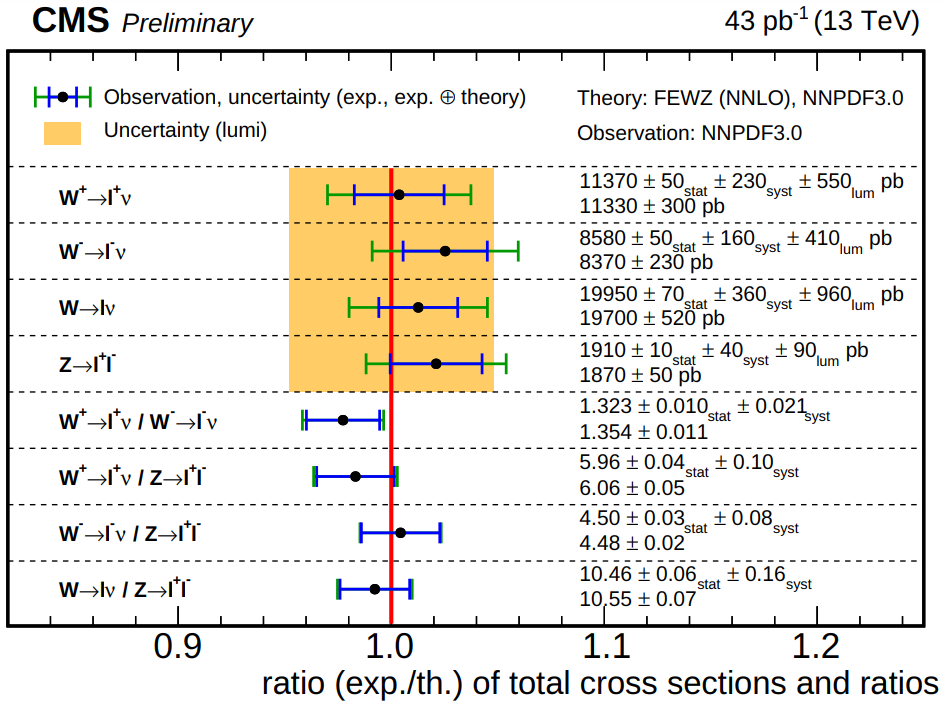
\includegraphics[scale=.28]{Chapter1/lumi_uncertainty.png} 
 \caption[Incertidumbre de la Luminosidad en un proceso]{Producción de bosones $W^+$, $W^-$, $W$ y $Z$ y sus predicciones teoricas. La caja sombreada indica las incertidumbres en la medición de la luminosidad, mostrando que estas son mayores que las incertidumbres experimentales (barras azules) y las incertidumbres teóricas (barras verdes). Los valores de las mediciones y las predicciones teóricas se encuentran en la parte derecha de la figura.}
    \label{lumi_incertainty}
  \end{figure}
\end{center}


\section{El Gran Colisionador de Hadrones (LHC)}
 
El Gran Colisionador de Hadrones (LHC) es el acelerador de partículas más grande y potente del mundo. Comenzó a operar el 10 de septiembre de 2008 y es la adición más reciente al complejo de aceleradores de CERN. El LHC consta de un anillo de 27 kilómetros que contiene imanes superconductores, además de varias estructuras utilizadas para acelerar las partículas mientras se desplazan a lo largo del anillo. Dentro del acelerador, dos haces de partículas viajan a velocidades cercanas a la de la luz hasta que colisionan. Los haces se mueven en direcciones opuestas dentro de tubos separados, que se mantienen en un vacío ultra alto \cite{LHC}.\\ 

Los electroimanes superconductores generan un potente campo magnético que guía los haces de partículas a lo largo del anillo del acelerador. Estos imanes están formados por bobinas de un cable eléctrico especial que funciona en un estado superconductor. En este estado, el cable puede conducir electricidad sin resistencia ni pérdida de energía. El acelerador utiliza una variedad de imanes, entre ellos 1232 imanes dipolares de 15 metros de longitud que desvían los haces, y 392 imanes cuadrupolares de entre 5 y 7 metros de longitud que enfocan los haces. Justo antes de la colisión, se emplea un tipo diferente de imán para "comprimir" las partículas, aumentando así la probabilidad de colisiones. Para mantener estos imanes en estado superconductor, deben ser enfriados a una temperatura extremadamente baja de -271.3°C.\\

El proceso de generar haces de protones para el LHC es complejo y se lleva a cabo en varias etapas. Primero, se ioniza el hidrógeno para obtener protones, los cuales son acelerados en paquetes hasta alcanzar una energía de $50 MeV$ en el Acelerador Lineal 2 (LINAC2). Posteriormente, estos paquetes pasan por tres aceleradores circulares: el Booster, el Sincrotrón de Protones (PS) y el Super Sincrotrón de Protones (SPS), donde se aumenta su energía gradualmente a $1.4 GeV, 26 GeV$ y $450 GeV$, respectivamente. Después de estas fases de preaceleración, los paquetes de protones son inyectados en el anillo del LHC, donde se aceleran aún más hasta alcanzar energías de hasta $7 TeV$ por paquete, mientras circulan en direcciones opuestas. Este ciclo se denomina un "llenado" del LHC y generalmente involucra alrededor de \(10^{14}\) protones, organizados en paquetes que forman el haz de protones. La figura 1.4 muestra una representación esquemática de todo el complejo de aceleradores del CERN.

\begin{center}
  \begin{figure}[h]
    \centering
    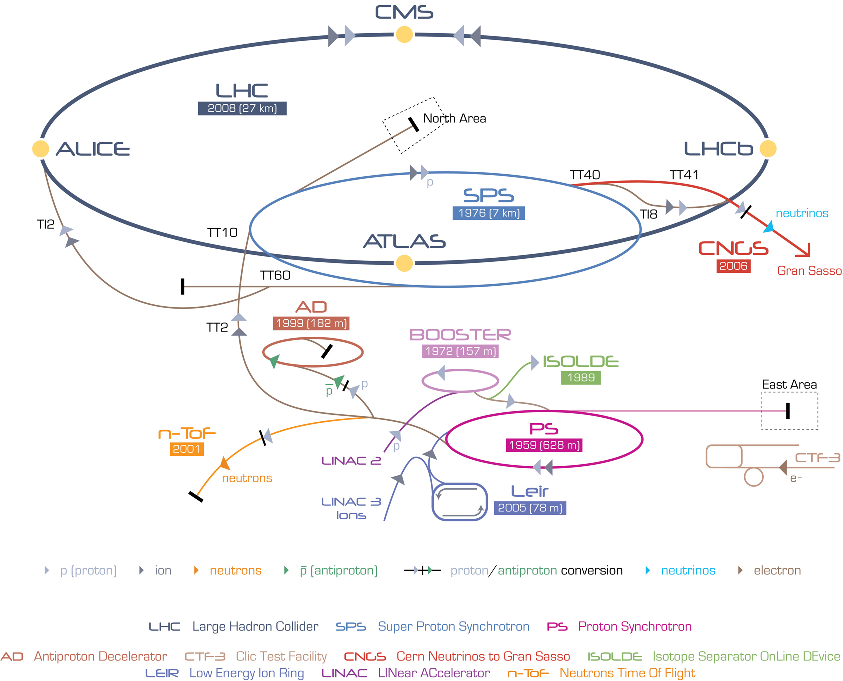
\includegraphics[scale=.35]{Chapter1/lhc_complex_fig.png}
    \caption[Complejo LHC]{Diagrama de llenado del LHC.}
    \label{lhc_com}
  \end{figure}
\end{center}

El Centro de Control del CERN es el centro neurálgico encargado de gestionar todos los controles, servicios e infraestructura técnica del LHC. Desde allí, se dirigen los haces de protones para que colisionen en cuatro ubicaciones diferentes a lo largo del anillo del acelerador, las cuales corresponden a las posiciones de cuatro detectores de partículas. CMS y ATLAS son detectores de propósito general diseñados para explorar una amplia variedad de física del Modelo Estándar (SM) y más allá del Modelo Estándar (BSM), mientras que ALICE y LHCb son detectores especializados que se centran en el estudio de fenómenos específicos.

